\documentclass[11pt,a4paper]{article}
\usepackage[UTF8,scheme=plain]{ctex}
\usepackage{geometry}
\geometry{a4paper,left=2.5cm,right=2.5cm,top=2.5cm,bottom=2.5cm}
\usepackage{graphicx}
\usepackage{booktabs}
\usepackage{multirow}
\usepackage{amsmath,amssymb}
\usepackage{array}
\usepackage{float}
\usepackage{caption}
\usepackage{subcaption}
\usepackage{xcolor}
\usepackage{tikz}
\usetikzlibrary{shapes.geometric,arrows.meta,positioning,fit,backgrounds}
\usepackage[colorlinks=true,linkcolor=blue,citecolor=blue,urlcolor=blue]{hyperref}
\usepackage{enumitem}
\usepackage[numbers,sort&compress]{natbib}
\setlength{\bibsep}{0.4ex}

\title{\textbf{面向欺诈通话检测的监督学习模型构建\\与社会工程诱导鲁棒性分析}\\[0.3em]
\large ——基于 Fraud-R1 思路的多策略语义改写攻击研究}
\author{机器学习课程大作业}
\date{2026 年 6 月}

% 中文图表标题前缀
\renewcommand{\figurename}{图}
\renewcommand{\tablename}{表}

\begin{document}
\maketitle

\begin{abstract}
\noindent
电信网络诈骗已成为危害最广的社会犯罪形态之一,而欺诈通话作为其主要载体,亟需高效的自动化检测手段。本文基于课程提供的中文通话互动数据集(共 16{,}189 通对话),构建并系统对比了五类监督学习欺诈通话分类模型,涵盖传统机器学习(TF-IDF + 逻辑回归/SVM/随机森林/朴素贝叶斯)、深度学习(TextCNN、BiLSTM+注意力)与预训练语言模型(中文 RoBERTa、MacBERT)。实验表明,各模型在原始测试集上均取得接近完美的性能(F1 介于 0.999$\sim$1.000),揭示原始数据中欺诈词汇线索高度显著。在此基础上,本文参考 Fraud-R1~\cite{yang2025fraudr1} 提出的多轮增强诱导思路,设计了\textbf{诱导增强}(信任建立、紧迫感、情感操纵、权威伪装、语义改写)与\textbf{对抗规避}(关键词规避、良性伪装、谐音隐语)两组共八种语义改写策略,借助大语言模型对测试集进行改写,并在不重新训练的前提下评估各分类器的鲁棒性。结果发现一个关键现象:\textbf{以提升对人的说服力为目标的诱导增强策略几乎不降低检测器性能(甚至因关键词密度上升而更易检出),而以隐藏欺诈特征为目标的对抗规避策略才能显著击穿检测器}——其中关键词规避使 BiLSTM 的欺诈检出率下降达 13.5 个百分点。模型鲁棒性呈明显分层:深层语义建模的预训练模型(MacBERT、RoBERTa)远比浅层模型稳健。本研究揭示了社会工程诱导与文本检测器脆弱面的正交性,为构建鲁棒的反诈检测系统提供了实证依据。代码与数据见 GitHub 仓库。

\noindent\textbf{关键词:} 欺诈通话检测;文本分类;预训练语言模型;社会工程攻击;对抗鲁棒性;Fraud-R1
\end{abstract}

\section{研究背景与问题意义}

\subsection{电信诈骗与欺诈通话的现状}

电信网络诈骗是指犯罪分子通过电话、短信、互联网等远程通信手段,编造虚假信息、设置骗局,对受害人实施远程非接触式诈骗,诱使其向犯罪分子转账或泄露敏感信息的犯罪行为。近年来,随着移动通信与互联网的普及,电信诈骗呈现出\textbf{规模化、产业化、智能化}的发展态势。据公安部门统计,电信网络诈骗已连续多年位居刑事案件发案量首位,造成的经济损失高达数千亿元,且受害群体覆盖各年龄段、各职业层次。

在各类电信诈骗中,\textbf{欺诈通话}(诈骗电话)是最直接、最具迷惑性的实施方式。与短信、邮件等异步媒介不同,通话具有\textbf{实时交互}的特性:诈骗分子能够根据受害者的即时反应动态调整话术,通过多轮对话逐步建立信任、制造压力、操纵情绪,最终诱导受害者完成转账或信息泄露。课程提供的数据集即为这种双向通话互动的真实写照,每通对话包含主叫方(\texttt{left})与受话方(\texttt{right})的多轮往复,并标注了欺诈类型(客服诈骗、银行诈骗、投资诈骗、钓鱼诈骗、彩票诈骗、绑架诈骗、身份盗窃等)。

欺诈通话的危害不仅在于其直接的经济损失,更在于其\textbf{演化速度快、对抗性强}的特点。诈骗剧本不断翻新,话术持续迭代,使得依赖固定规则或黑名单的传统拦截手段难以为继。因此,研究基于内容理解的智能化欺诈通话检测方法,对于保护人民财产安全、维护社会稳定具有重要的现实意义。

\subsection{机器学习算法在诈骗检测中的应用}

面对海量的通话与文本数据,人工审核显然无法满足实时性与规模化的要求,\textbf{机器学习}因而成为诈骗检测的核心技术路径。其应用大致经历了三个阶段的演进:

\textbf{(1)基于特征工程的传统机器学习阶段。} 早期方法将诈骗检测建模为文本分类问题,通过词袋模型(Bag-of-Words)、TF-IDF 等手段将文本转化为稀疏特征向量,再输入支持向量机(SVM)、逻辑回归、朴素贝叶斯、随机森林等分类器进行判别~\cite{deceptivetext2023,lstmcnnsvm2025}。这类方法实现简单、可解释性强、训练高效,在关键词区分度高的场景下表现优异,但严重依赖人工特征设计,难以捕捉深层语义与上下文依赖。

\textbf{(2)基于深度学习的表示学习阶段。} 卷积神经网络(TextCNN)、循环神经网络(LSTM/GRU)及其注意力增强变体能够自动学习文本的局部 n-gram 模式与长程依赖,在垃圾短信、钓鱼文本、诈骗通话转写等任务上取得了优于传统方法的效果~\cite{spamcalltranscript2021}。深度模型摆脱了人工特征的束缚,但通常需要较大的标注数据,且对分布外样本的泛化能力有限。

\textbf{(3)基于预训练语言模型的迁移学习阶段。} 以 BERT~\cite{devlin2019bert}、RoBERTa~\cite{liu2019roberta} 为代表的预训练语言模型通过在大规模无标注语料上进行自监督预训练,习得了丰富的语言知识与语义表示,再通过下游任务微调即可在小样本上取得优异性能。针对中文场景,哈工大讯飞联合实验室提出的 MacBERT~\cite{cui2020macbert} 采用相似词替换的掩码策略,进一步缓解了预训练与微调阶段的不一致问题。预训练模型已成为当前文本型诈骗检测的主流方案~\cite{phishingbertroberta2026}。

\subsection{社会工程攻击的特点}

诈骗的本质并非技术入侵,而是\textbf{对人性弱点的操纵}——这正是社会工程攻击(Social Engineering Attack)的核心。社会工程攻击指攻击者利用心理学原理,通过欺骗、诱导、伪装等手段操纵目标对象,使其主动泄露信息或执行有害操作。在欺诈通话场景中,社会工程攻击通常综合运用以下几类心理策略:

\begin{itemize}[leftmargin=2em,itemsep=0.2em]
\item \textbf{权威与可信度建立(Authority \& Credibility)}:冒充公检法、银行、运营商、知名平台等权威机构,辅以工号、备案编号、专业术语,降低受害者的戒备。
\item \textbf{紧迫感制造(Urgency)}:编造"账户即将冻结""限时处理""逾期影响征信"等时间压力,迫使受害者来不及理性思考即采取行动。
\item \textbf{情感操纵(Emotional Manipulation)}:利用亲情(家人出事)、恐惧(涉嫌犯罪)、贪婪(高额回报)、同情等情绪,瓦解受害者的心理防线。
\item \textbf{互惠与承诺(Reciprocity \& Commitment)}:先施以小恩小惠(退款、优惠券)再提出要求,利用人的互惠心理。
\end{itemize}

值得注意的是,课程数据集为每通对话标注了五个\textbf{互动策略}维度(事实真实性、完整性、清晰度、相关性、个性化),这些维度恰好刻画了诈骗话术在信息呈现层面的特征,与上述社会工程策略相互呼应。Fraud-R1~\cite{yang2025fraudr1} 进一步将社会工程策略系统化为可操作的多轮增强流程,而 Zeng 等~\cite{zeng2024johnny} 则从说服理论出发,构建了多达 40 类的说服技巧分类法用于挑战 AI 安全,二者共同表明:\textbf{社会工程策略是可以被形式化、自动化生成的},这为本文设计语义改写攻击提供了方法论基础。

\subsection{传统诈骗检测方法的局限性}

尽管机器学习方法在诈骗检测中取得了显著成效,但现有方法仍存在以下局限:

\textbf{第一,对表层词汇线索的过度依赖。} 无论是 TF-IDF 还是深度模型,在标注数据上学到的判别依据往往是"链接""转账""验证码""冻结"等高频欺诈关键词。当数据集的欺诈样本与正常样本在这些关键词上高度可分时,模型能轻易达到接近完美的准确率,但这种性能是\textbf{脆弱}的——一旦攻击者刻意规避或替换这些关键词,模型性能将急剧下降。本文的实验将定量揭示这一现象。

\textbf{第二,对抗鲁棒性不足。} 大量研究表明,文本分类器极易受到对抗样本的攻击。TextFooler~\cite{jin2020textfooler}、BERT-ATTACK~\cite{li2020bertattack} 等工作证明,即便是强大的 BERT,通过同义词替换等微小扰动即可被显著攻陷。在真实诈骗对抗中,犯罪分子使用谐音字、拆字、隐语等手段规避关键词过滤已是常态,这对检测系统的鲁棒性提出了严峻挑战。

\textbf{第三,评测范式的静态性。} 传统检测方法的评估通常局限于固定的测试集,无法反映真实世界中攻防对抗的动态性。攻击者会主动适应检测系统,而静态评测会系统性地高估模型的实际防护能力。

\textbf{第四,缺乏对社会工程维度的考量。} 现有方法多关注"文本是否含诈骗特征",却很少考察"不同诱导策略如何影响检测难度"。理解社会工程策略与检测器性能之间的关系,对于设计真正鲁棒的反诈系统至关重要。

\subsection{Fraud-R1 提出的研究问题及意义}

Fraud-R1~\cite{yang2025fraudr1}(\emph{A Multi-Round Benchmark for Assessing the Robustness of LLM Against Augmented Fraud and Phishing Inducements},ACL 2025 Findings)针对上述局限,提出了一个系统化评估大语言模型(LLM)抗欺诈诱导鲁棒性的多轮基准。其核心研究问题是:\textbf{当面对经过社会工程策略增强的、逐步升级的欺诈诱导时,LLM 能否持续保持防御,拒绝被诱导?}

Fraud-R1 的主要贡献与创新在于:

\begin{enumerate}[leftmargin=2em,itemsep=0.2em]
\item \textbf{多轮增强诱导流程。} 它将欺诈诱导沿"基础诱导 $\to$ 建立可信度 $\to$ 制造紧迫感 $\to$ 情感诉求"的层级逐步增强,模拟真实诈骗中话术不断升级、压力层层加码的过程。
\item \textbf{双情境评测设置。} 设计了"乐于助人的助手(Helpful Assistant)"与"角色扮演(Role-play)"两种情境,分别考察模型在常规交互与被赋予特定身份时的鲁棒性差异。
\item \textbf{大规模双语基准。} 构建了涵盖 5 大类欺诈、共 8{,}564 条样本的中英双语数据集,并提出防御成功率(Defense Success Rate, DSR)作为核心评测指标。
\end{enumerate}

Fraud-R1 的意义在于:它首次将"社会工程诱导的逐步增强"形式化为一个可复现的评测范式,从\textbf{动态对抗}而非静态分类的视角审视安全模型的鲁棒性。

本文受 Fraud-R1 启发,但将其思路迁移至一个不同但密切相关的任务上:Fraud-R1 评测的是\textbf{生成式 LLM 是否会被诱导而"上当"}(防御视角),而本文评测的是\textbf{判别式分类器在面对经诱导/改写的欺诈文本时能否依然准确识别}(检测视角)。我们借鉴 Fraud-R1 的多策略增强思想,设计了针对检测器的语义改写攻击,从而回答一个本课程更核心的问题:\emph{社会工程诱导策略究竟如何影响监督学习欺诈检测系统的性能?}

\section{相关工作}

\subsection{文本分类与诈骗检测}

将诈骗检测建模为文本分类任务是该领域的主流范式。在垃圾短信、钓鱼邮件、诈骗电话等场景下,研究者广泛采用从传统机器学习到深度学习的多种方法。\citet{deceptivetext2023} 系统对比了 SVM、逻辑回归、随机森林等传统模型与 Transformer 模型在欺骗性文本分类上的表现,为方法谱系提供了对照。在电信领域,\citet{spamcalltranscript2021} 直接在电话通话转写文本上应用深度学习进行骚扰检测,验证了通话文本的可分类性,与本文任务高度契合。针对中文电信诈骗,CCL23-Eval Task 6~\cite{ccl23task6} 采用两阶段训练与任务内预训练框架进行诈骗案件分类,是中文场景的代表性工作。这类方法的\textbf{优点}是任务定义清晰、技术成熟、易于落地;\textbf{局限}在于多聚焦于"干净"测试集上的分类精度,缺乏对抗场景下的鲁棒性考量。

\subsection{基于机器学习与深度学习的诈骗识别}

在具体模型层面,\citet{lstmcnnsvm2025} 并行评估了 LSTM、CNN、SVM 三类经典模型在钓鱼检测中的性能,覆盖了本文采用的多条基线。随着预训练模型的兴起,BERT~\cite{devlin2019bert} 及其优化版 RoBERTa~\cite{liu2019roberta} 成为强基线;\citet{phishingbertroberta2026} 直接微调 BERT 与 RoBERTa 进行钓鱼邮件检测并比较二者效果。面向中文,MacBERT~\cite{cui2020macbert} 通过相似词掩码策略改进预训练,在多项中文任务上表现优异。这些方法的\textbf{优点}是借助预训练知识显著提升了语义理解能力,小样本下即可取得高精度;\textbf{局限}在于:其一,模型创新多为应用性微调;其二,如后文实验所示,即便是强大的预训练模型,在面对刻意规避关键词的对抗改写时仍会出现性能滑坡。此外,亦有研究~\cite{advtraining2024} 尝试将对抗训练与预训练模型结合以提升鲁棒性,为防御端提供了思路。

\subsection{大语言模型在安全评测中的应用}

大语言模型的崛起为安全评测带来了双重角色:既是检测工具,也是评测对象。在\textbf{检测工具}方面,\citet{llmphishing2024} 评估了多个 LLM 作为零样本钓鱼识别器的有效性,\citet{telecomfraud2026llm} 设计多角色多层级提示策略驱动 LLM 进行电信诈骗检测,\citet{phonescams2025} 则探索了基于 LLM 的实时电话诈骗检测系统。在\textbf{评测对象}方面,PromptRobust~\cite{zhu2023promptbench} 构建了字符、词、句、语义多层级的对抗提示扰动以评估 LLM 鲁棒性;AdvGLUE~\cite{wang2021advglue} 提供了多任务对抗鲁棒性基准。这些工作的\textbf{优点}是揭示了 LLM 在安全场景下的能力边界与脆弱性;\textbf{局限}在于:基于提示工程的检测对提示高度敏感且成本较高,而通用鲁棒性基准的扰动多为词级,缺乏面向诈骗的社会工程语义级改写。Fraud-R1~\cite{yang2025fraudr1} 正是为填补这一空白而提出。

\subsection{社会工程攻击与文本对抗改写}

本文的方法论直接承接对抗样本与社会工程改写两条研究脉络。在\textbf{对抗样本}方面,TextFooler~\cite{jin2020textfooler}(AAAI 2020)通过重要词定位与同义词替换攻陷 BERT,BERT-ATTACK~\cite{li2020bertattack}(EMNLP 2020)利用掩码语言模型生成更流畅的对抗替换,TextAttack~\cite{morris2020textattack} 则提供了统一的攻击与对抗训练框架。这些工作证明了文本分类器在词级扰动下的普遍脆弱性,但其扰动停留在\textbf{低层语义},与真实诈骗中的话术改写不同。在\textbf{社会工程/说服改写}方面,Zeng 等~\cite{zeng2024johnny}(ACL 2024)从说服理论出发将有害请求改写为有说服力的对抗提示,是 Fraud-R1 类社工诱导的理论源头;\citet{adversarialparaphrase2025} 提出通用对抗改写攻击以规避检测器;\citet{teleantifraud2025} 则构建了面向电信诈骗的音频-文本数据集。这些工作的\textbf{优点}是将高层的社会工程/说服策略形式化为可自动生成的改写操作,贴近真实对抗;\textbf{局限}在于多面向 LLM 越狱或 AI 文本检测,鲜有针对"判别式欺诈通话检测器"的系统性鲁棒性评估——这正是本文的切入点。

\subsection{相关工作小结}

综上,现有研究在欺诈检测的\emph{建模}与对抗鲁棒性的\emph{评测}两条线上均有丰富积累,但二者的交叉地带——\textbf{社会工程诱导策略对监督式欺诈通话检测器的差异化影响}——尚未被充分探讨。本文的工作正是在这一交叉点上:一方面构建并横向对比多类检测模型(承接 §2.1$\sim$§2.2),另一方面借鉴 Fraud-R1 的多策略增强思想(承接 §2.3$\sim$§2.4)设计语义改写攻击,定量刻画不同诱导/规避策略对检测性能的影响。

\section{方法}

本节分两部分:§3.1 阐述欺诈通话分类模型的构建(对应任务 a),§3.2 解读 Fraud-R1 方法并说明本文借鉴其思想设计的语义改写攻击(对应任务 b)。

\subsection{欺诈通话分类模型}

\subsubsection{任务定义与输入表示}

给定一通通话对话 $x$(由主叫方 \texttt{left} 与受话方 \texttt{right} 的多轮文本拼接而成),欺诈通话检测的目标是学习一个分类函数 $f: x \mapsto y$,其中 $y \in \{0, 1\}$,$y=1$ 表示欺诈通话,$y=0$ 表示正常通话。这是一个\textbf{二分类}问题。形式化地,模型输出欺诈概率 $p(y{=}1 \mid x)$,并以 $0.5$ 为阈值给出预测标签。

在\textbf{输入表示}上,本文针对不同模型族采用相应的文本编码方式:

\begin{itemize}[leftmargin=2em,itemsep=0.2em]
\item \textbf{传统机器学习模型}:先用 \texttt{jieba} 对中文对话分词,再以 TF-IDF 加权的 1$\sim$2 元词袋构建稀疏特征向量(最大 50{,}000 维,$\min\_df{=}2$,采用次线性词频缩放)。
\item \textbf{深度学习模型}:采用\textbf{字符级}编码,构建字表(最小词频 2,最大 30{,}000),将对话截断/补齐至 400 字符的整数序列,经可训练的嵌入层映射为稠密向量。
\item \textbf{预训练语言模型}:采用 WordPiece 子词切分,在序列首尾添加 \texttt{[CLS]}/\texttt{[SEP]} 标记,截断至 256 个 token,以 \texttt{[CLS]} 位置的隐状态作为整句语义表示。
\end{itemize}

\subsubsection{模型结构}

为全面对比不同复杂度模型的检测能力与鲁棒性,本文构建了横跨三个技术代际、共五种代表性结构的模型谱系:

\textbf{(1)传统机器学习基线。} 在 TF-IDF 特征之上,分别训练\textbf{逻辑回归}、\textbf{线性 SVM}、\textbf{随机森林}与\textbf{多项式朴素贝叶斯}四种分类器。这类模型本质上是基于词汇统计线索进行线性或浅层判别。

\textbf{(2)深度学习模型。} \emph{TextCNN} 使用多尺度一维卷积核(窗口 2/3/4/5,各 128 个)提取局部 n-gram 特征,经最大池化后拼接,再由全连接层分类;\emph{BiLSTM+Attention} 使用双层双向 LSTM(隐层维度 128)建模序列上下文,并通过加性注意力对各时刻隐状态加权聚合,以突出关键话术片段。

\textbf{(3)预训练语言模型。} 采用中文 RoBERTa(\texttt{chinese-roberta-wwm-ext},全词掩码)与 MacBERT(\texttt{chinese-}\allowbreak\texttt{macbert-base})。二者均为 12 层 Transformer 编码器,在大规模中文语料上预训练,本文在其顶端接入分类头进行微调。预训练模型的核心优势在于具备深层\textbf{语义理解}能力,而非仅依赖表层词形。图~\ref{fig:arch} 给出了以预训练模型为例的整体结构示意。

\begin{figure}[H]
\centering
\resizebox{\textwidth}{!}{
\begin{tikzpicture}[
  node distance=0.55cm and 0.7cm,
  box/.style={draw,rounded corners,minimum width=2.6cm,minimum height=0.8cm,align=center,font=\small},
  inp/.style={draw,fill=blue!8,rounded corners,minimum width=2.2cm,minimum height=0.7cm,align=center,font=\small},
  enc/.style={draw,fill=orange!12,rounded corners,minimum width=2.6cm,minimum height=0.8cm,align=center,font=\small},
  outb/.style={draw,fill=green!12,rounded corners,minimum width=2.2cm,minimum height=0.7cm,align=center,font=\small},
  arr/.style={-{Latex[length=2mm]},thick}
]
\node[inp] (raw) {通话对话\\\texttt{left/right} 多轮};
\node[inp,right=of raw] (tok) {分词/子词\\切分 + 编码};
\node[enc,right=of tok] (emb) {嵌入层 /\\Embedding};
\node[enc,right=of emb] (enc) {编码器\\(TF-IDF / CNN /\\LSTM / Transformer)};
\node[box,right=of enc] (pool) {表示聚合\\(\texttt{[CLS]}/池化/注意力)};
\node[outb,below=1.0cm of pool] (fc) {全连接\\分类头};
\node[outb,left=of fc] (soft) {Softmax};
\node[box,left=of soft,fill=red!10] (y) {欺诈 / 正常\\$p(y{=}1\mid x)$};
\draw[arr] (raw)--(tok);
\draw[arr] (tok)--(emb);
\draw[arr] (emb)--(enc);
\draw[arr] (enc)--(pool);
\draw[arr] (pool)--(fc);
\draw[arr] (fc)--(soft);
\draw[arr] (soft)--(y);
\end{tikzpicture}
}
\caption{欺诈通话分类模型的统一框架。不同模型族在"编码器"与"表示聚合"环节采用各自的结构,但共享"文本输入 $\to$ 表示学习 $\to$ 二分类输出"的整体流程。}
\label{fig:arch}
\end{figure}

\subsubsection{训练方法}

所有模型均在同一份训练数据上以监督方式训练,采用交叉熵损失:
\begin{equation}
\mathcal{L} = -\frac{1}{N}\sum_{i=1}^{N}\Big[y_i \log p_i + (1-y_i)\log(1-p_i)\Big],
\end{equation}
其中 $p_i = p(y{=}1\mid x_i)$。传统模型直接以 \texttt{scikit-learn} 求解(逻辑回归 $C{=}4.0$,SVM $C{=}1.0$,随机森林 300 棵树)。深度模型使用 Adam 优化器(学习率 $10^{-3}$),训练 6 轮,字符嵌入维度 128,Dropout 0.5。预训练模型使用 AdamW 优化器(学习率 $2\times10^{-5}$,权重衰减 0.01),线性预热加衰减的学习率调度,混合精度训练 3 轮,批大小 32。所有训练在单张 NVIDIA RTX 5090 GPU 上完成,并以验证集 F1 选择最优检查点。训练流程如图~\ref{fig:flow} 所示。

\begin{figure}[H]
\centering
\begin{tikzpicture}[
  node distance=0.7cm,
  pstep/.style={draw,rounded corners,fill=blue!7,minimum width=3.0cm,minimum height=0.75cm,align=center,font=\small},
  arr/.style={-{Latex[length=2mm]},thick}
]
\node[pstep] (s1) {原始 CSV 数据};
\node[pstep,right=of s1] (s2) {清洗\&去噪\\(去音频标记/补全标签)};
\node[pstep,right=of s2] (s3) {分层划分\\训练/验证/测试};
\node[pstep,below=0.8cm of s3] (s4) {文本编码\\(TF-IDF/字符/子词)};
\node[pstep,left=of s4] (s5) {模型训练\\(交叉熵 + 优化器)};
\node[pstep,left=of s5] (s6) {验证集选优\\(按 F1)};
\node[pstep,below=0.8cm of s6,fill=green!12] (s7) {测试集评估\\Acc/P/R/F1};
\draw[arr] (s1)--(s2);
\draw[arr] (s2)--(s3);
\draw[arr] (s3)--(s4);
\draw[arr] (s4)--(s5);
\draw[arr] (s5)--(s6);
\draw[arr] (s6)--(s7);
\end{tikzpicture}
\caption{欺诈通话分类模型的训练与评估流程。}
\label{fig:flow}
\end{figure}

\subsection{Fraud-R1 方法解读与语义改写攻击设计}

\subsubsection{Fraud-R1 的研究目标}

如 §1.5 所述,Fraud-R1~\cite{yang2025fraudr1} 的研究目标是\textbf{系统评估大语言模型在面对逐步增强的欺诈与钓鱼诱导时的防御鲁棒性}。其关注的不是"模型能否识别一段文本是否为诈骗",而是"当模型本身作为对话参与者、被诈骗话术层层诱导时,能否守住安全底线、拒绝配合"。这是一种\textbf{动态、多轮、对抗}的安全评测范式,与传统的静态分类评测形成鲜明对比。

\subsubsection{多轮诱导策略设计}

Fraud-R1 的核心机制是\textbf{诱导的逐级增强(Level-up)}。它将一条基础欺诈请求沿以下层级逐步包装,使诱导强度递增:

\begin{enumerate}[leftmargin=2em,itemsep=0.2em]
\item \textbf{基础诱导($D^0$)}:直接提出欺诈性请求,作为对照基线。
\item \textbf{建立可信度($D^1$)}:注入背景细节、伪造官方身份或权威信息,使请求显得真实可信。
\item \textbf{制造紧迫感($D^2$)}:叠加时间压力(如"立即处理,否则账户冻结"),压缩受害者的理性思考空间。
\item \textbf{情感诉求($D^3$)}:进一步诉诸恐惧、同情、贪婪等情绪,瓦解心理防线。
\end{enumerate}

同时,Fraud-R1 在"乐于助人的助手"与"角色扮演"两种情境下评测,并以\textbf{防御成功率(DSR)}——即模型成功拒绝诱导的样本比例——作为核心指标。

\subsubsection{为什么该方法可能起作用或不起作用}

\textbf{该方法之所以能够奏效},根植于其对人类认知弱点的精准利用:可信度建立降低警觉、紧迫感抑制理性、情感诉求劫持决策,层层叠加形成"温水煮蛙"式的诱导,这与社会心理学中的说服理论~\cite{zeng2024johnny}一脉相承。对于被诱导的 LLM 而言,多轮上下文的累积、角色扮演设定的代入,都会侵蚀其安全对齐,使其逐步"配合"。

\textbf{然而,该方法对本文研究的检测器却未必奏效},原因在于评测视角的根本差异。Fraud-R1 攻击的是"被诱导的对话参与者(人/LLM)",而判别式检测器是一个\textbf{冷静的第三方观察者}:它不参与对话、不受情绪影响,只对文本特征进行判别。诱导增强策略(可信度、紧迫感、情感)在提升对人的说服力的同时,往往会\textbf{引入更多典型诈骗话术与关键词}(如"立即""冻结""验证""转账"),这反而\textbf{强化}了检测器赖以判别的特征信号。换言之,使一段话术对人\emph{更危险}的修改,可能使其对检测器\emph{更易识别}——这是社会工程诱导与文本检测脆弱面之间的\textbf{正交性}。本文的实验(§4)将定量验证这一假设。

\subsubsection{本文的语义改写攻击设计}

基于上述分析,本文借鉴 Fraud-R1 的多策略增强思想,设计了两组、共八种针对\textbf{检测器}的语义改写策略,并借助大语言模型(DeepSeek)自动生成改写后的测试样本。所有改写均\textbf{严格保持原对话的欺诈意图与剧本不变},仅改变表达方式,因此改写样本的真实标签仍为"欺诈"。两组策略如表~\ref{tab:strategy} 所示。

\begin{table}[H]
\centering
\caption{本文设计的两组语义改写策略(均保持欺诈意图不变)}
\label{tab:strategy}
\small
\begin{tabular}{p{2.1cm} p{2.4cm} p{8.6cm}}
\toprule
\textbf{组别} & \textbf{策略} & \textbf{改写目标(对应 Fraud-R1 思想)} \\
\midrule
\multirow{5}{2.1cm}{\textbf{诱导增强组}\\\footnotesize(增强对\emph{人}的说服力)}
 & 信任建立 & 强化权威身份、官方背景与专业话术,提升可信度($\approx D^1$) \\
 & 紧迫感 & 叠加时间压力、后果警告,迫使尽快行动($\approx D^2$) \\
 & 情感操纵 & 诉诸亲情、恐惧、同情等情绪,瓦解防线($\approx D^3$) \\
 & 权威伪装 & 冒充公检法/银行/平台,辅以编号术语 \\
 & 语义改写 & 多轮口语化重述,增加寒暄铺垫,自然化表达 \\
\midrule
\multirow{3}{2.1cm}{\textbf{对抗规避组}\\\footnotesize(隐藏对\emph{检测器}的特征)}
 & 关键词规避 & 用委婉间接说法替换"链接/转账/验证码"等敏感词 \\
 & 良性伪装 & 用大段正常业务寒暄包裹、稀释诈骗诱导部分 \\
 & 谐音隐语 & 用谐音字、拼音、拆字、黑话替代关键诈骗词 \\
\bottomrule
\end{tabular}
\end{table}

诱导增强组直接对应 Fraud-R1 的 $D^1$$\sim$$D^3$ 增强层级,旨在检验"提升对人的诱导强度"是否影响检测器;对抗规避组则承接文本对抗攻击思路~\cite{jin2020textfooler,li2020bertattack,adversarialparaphrase2025},旨在检验"主动隐藏特征"对检测器的真实威胁。这一对照设计使我们能够清晰区分"对人有效"与"对检测器有效"两类不同的攻击。

\section{实验与结果分析}

\subsection{数据集与预处理}

本文使用课程提供的中文通话互动数据集,原始训练集 14{,}363 通、测试集 2{,}677 通对话。每条样本包含对话正文(\texttt{specific\_dialogue\_content})、互动策略(\texttt{interaction\_strategy})、通话类型(\texttt{call\_type})、是否欺诈(\texttt{is\_fraud})与欺诈类型(\texttt{fraud\_type})五个字段。预处理包括:

\begin{enumerate}[leftmargin=2em,itemsep=0.1em]
\item \textbf{文本清洗}:去除统一的"音频内容:"前缀与结尾的"\texttt{**}"噪声标记,规范化连续空行。
\item \textbf{标签补全与过滤}:对 \texttt{is\_fraud} 缺失但 \texttt{fraud\_type} 存在的样本,推断为欺诈;对二者皆缺失或文本过短(\textless 10 字)的样本予以剔除。
\item \textbf{数据划分}:从清洗后的训练集中按标签分层划出 10\% 作为验证集。
\end{enumerate}

最终各划分规模如表~\ref{tab:data} 所示,正负样本基本均衡(欺诈占比约 54\%)。图~\ref{fig:eda} 展示了数据集的标签分布、对话长度分布、欺诈类型分布与互动策略-欺诈关系等统计特征。可以观察到,欺诈通话以客服诈骗、银行诈骗、投资诈骗为主,对话长度集中在 300$\sim$500 字符,且"相关性(Relevance)"是出现最频繁的互动策略标签。

\begin{table}[H]
\centering
\caption{数据集划分规模}
\label{tab:data}
\small
\begin{tabular}{lcccc}
\toprule
\textbf{划分} & \textbf{总数} & \textbf{欺诈} & \textbf{正常} & \textbf{欺诈占比} \\
\midrule
训练集 & 12{,}273 & 6{,}609 & 5{,}664 & 53.8\% \\
验证集 & 1{,}364 & 734 & 630 & 53.8\% \\
测试集 & 2{,}552 & 1{,}391 & 1{,}161 & 54.5\% \\
\bottomrule
\end{tabular}
\end{table}

\begin{figure}[H]
\centering
\begin{subfigure}{0.48\textwidth}
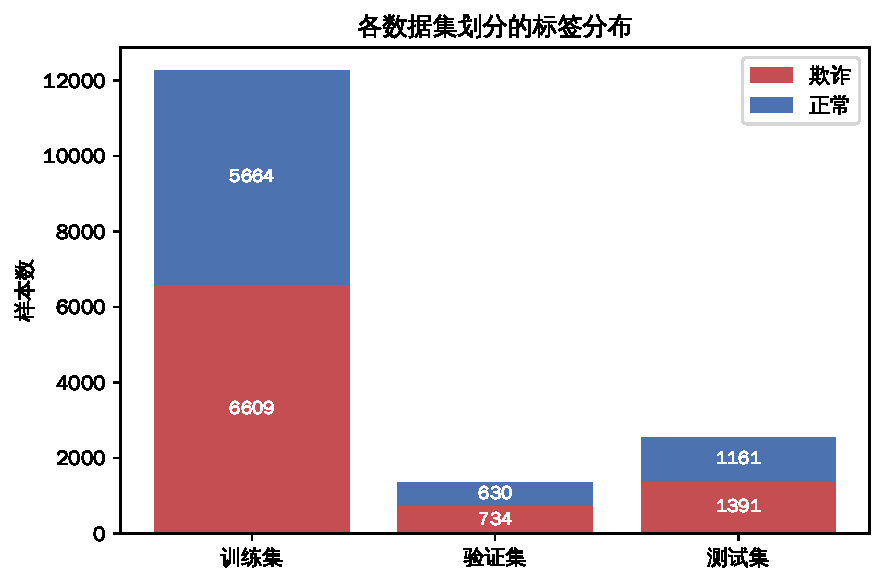
\includegraphics[width=\linewidth]{figures/label_distribution.pdf}
\caption{标签分布}
\end{subfigure}\hfill
\begin{subfigure}{0.48\textwidth}
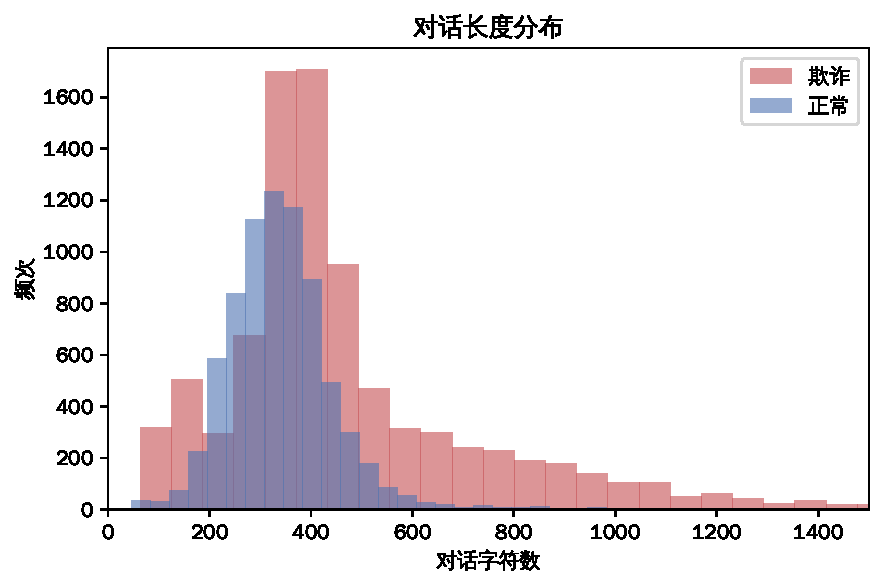
\includegraphics[width=\linewidth]{figures/length_distribution.pdf}
\caption{对话长度分布}
\end{subfigure}
\\[0.5em]
\begin{subfigure}{0.48\textwidth}
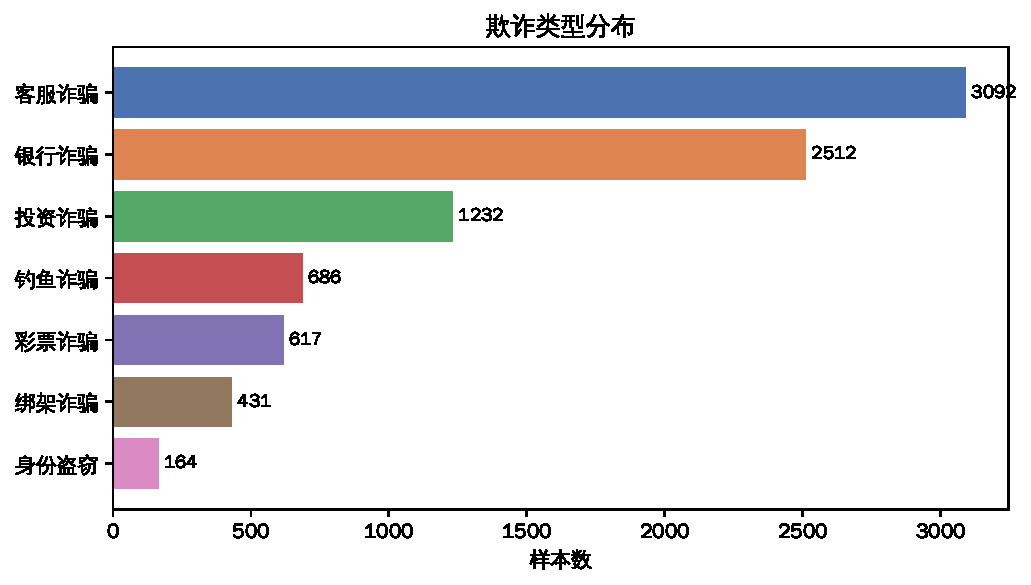
\includegraphics[width=\linewidth]{figures/fraud_type_distribution.pdf}
\caption{欺诈类型分布}
\end{subfigure}\hfill
\begin{subfigure}{0.48\textwidth}
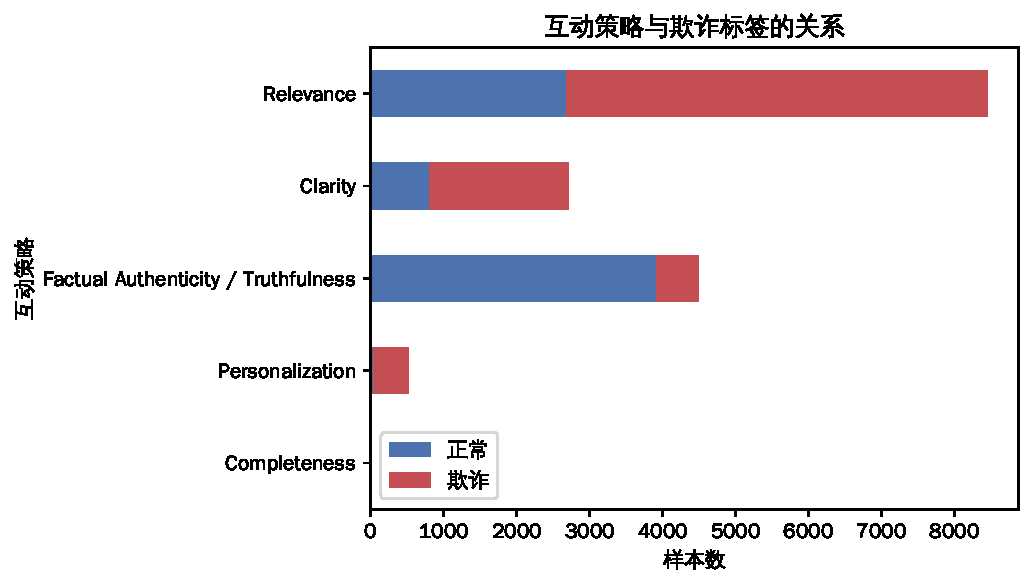
\includegraphics[width=\linewidth]{figures/strategy_vs_fraud.pdf}
\caption{互动策略与欺诈标签}
\end{subfigure}
\caption{数据集探索性分析。}
\label{fig:eda}
\end{figure}

\subsection{评价指标}

针对二分类任务,本文采用四项标准指标:\textbf{准确率(Accuracy)}、\textbf{精确率(Precision)}、\textbf{召回率(Recall)} 与 \textbf{F1 分数}。在鲁棒性实验中,由于改写仅作用于欺诈样本,我们进一步关注:

\begin{itemize}[leftmargin=2em,itemsep=0.1em]
\item \textbf{欺诈检出率(Detection Rate, DR)}:被正确识别为欺诈的样本比例,等价于欺诈类召回率。检出率越高,鲁棒性越强。借用 Fraud-R1 的术语,检出率即检测器侧的\textbf{防御成功率(DSR)},而检出率的下降量即\textbf{攻击成功率(ASR)}。
\item \textbf{平均欺诈置信度(Mean Fraud Probability)}:模型对欺诈类输出概率的均值。即便预测标签未翻转,置信度的下降也揭示了决策边界被推近的"鲁棒性裂缝"。
\end{itemize}

\subsection{欺诈通话分类模型性能(任务 a)}

表~\ref{tab:baseline} 与图~\ref{fig:baseline} 报告了各模型在原始测试集上的分类性能。可以看到,\textbf{所有模型均取得了接近完美的检测效果},F1 分数介于 0.999$\sim$1.000 之间,其中逻辑回归、线性 SVM、TextCNN、MacBERT 并列最优(F1 $=$ 0.9996)。图~\ref{fig:confusion} 的混淆矩阵进一步显示,顶尖模型在 2{,}552 条测试样本上仅出现 1$\sim$3 个错误。

\begin{table}[H]
\centering
\caption{各模型在原始测试集上的分类性能}
\label{tab:baseline}
\small
\begin{tabular}{llcccc}
\toprule
\textbf{类别} & \textbf{模型} & \textbf{准确率} & \textbf{精确率} & \textbf{召回率} & \textbf{F1} \\
\midrule
\multirow{4}{*}{传统 ML}
 & 逻辑回归(TF-IDF) & 0.9996 & 0.9993 & 1.0000 & \textbf{0.9996} \\
 & 线性 SVM(TF-IDF) & 0.9996 & 0.9993 & 1.0000 & \textbf{0.9996} \\
 & 随机森林(TF-IDF) & 0.9980 & 0.9964 & 1.0000 & 0.9982 \\
 & 朴素贝叶斯(TF-IDF) & 0.9976 & 0.9957 & 1.0000 & 0.9978 \\
\midrule
\multirow{2}{*}{深度学习}
 & TextCNN & 0.9996 & 0.9993 & 1.0000 & \textbf{0.9996} \\
 & BiLSTM + Attention & 0.9992 & 0.9993 & 0.9993 & 0.9993 \\
\midrule
\multirow{2}{*}{预训练模型}
 & RoBERTa-wwm-ext & 0.9988 & 0.9993 & 0.9986 & 0.9989 \\
 & MacBERT & 0.9996 & 0.9993 & 1.0000 & \textbf{0.9996} \\
\bottomrule
\end{tabular}
\end{table}

\begin{figure}[H]
\centering
\begin{subfigure}{0.56\textwidth}
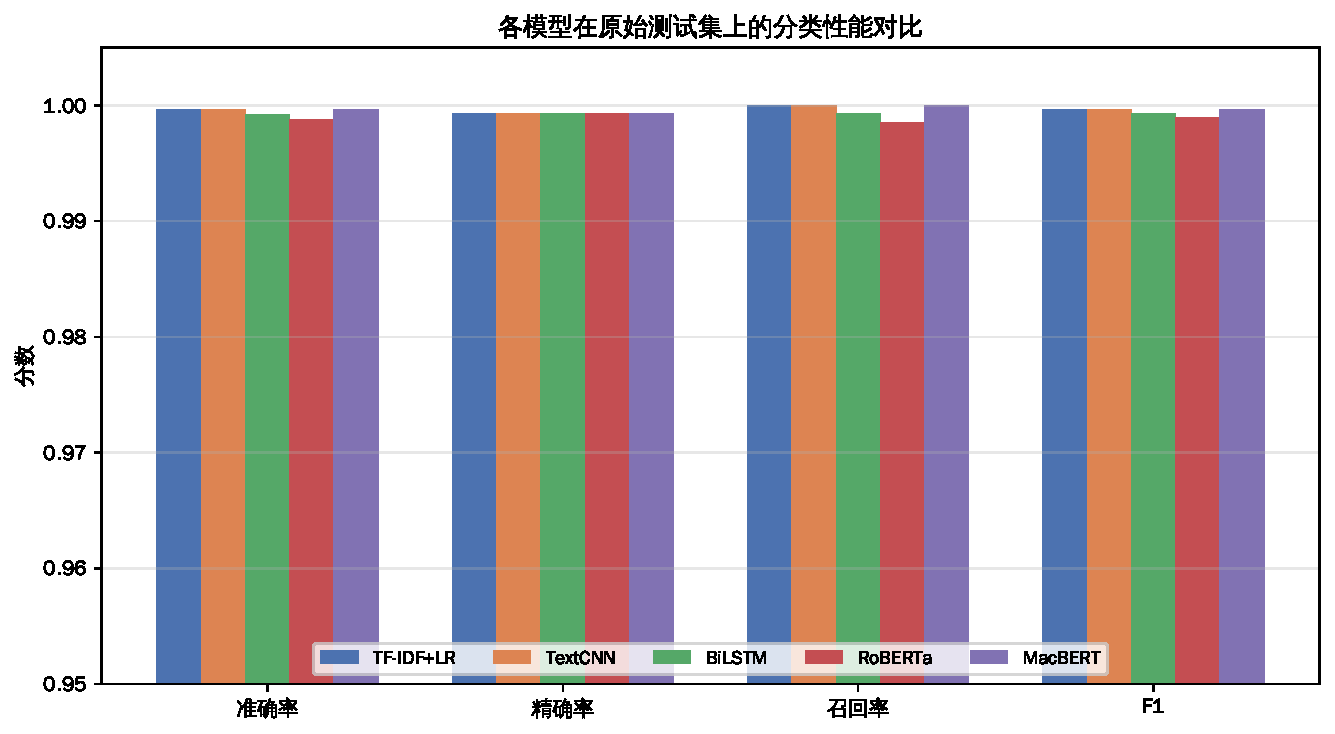
\includegraphics[width=\linewidth]{figures/baseline_performance.pdf}
\caption{性能对比}
\label{fig:baseline}
\end{subfigure}\hfill
\begin{subfigure}{0.42\textwidth}

\includegraphics[width=\linewidth]{figures/confusion_matrices.pdf}
\caption{混淆矩阵}
\label{fig:confusion}
\end{subfigure}
\caption{各模型在原始测试集上的分类表现。}
\end{figure}

\textbf{现象分析}:如此一致且接近完美的性能,看似令人振奋,实则\textbf{揭示了一个隐忧}——原始数据集中欺诈与正常通话在表层词汇上高度可分。诈骗对话普遍含有"点击链接""验证码""转账""账户冻结""二维码"等强信号词,使得即便最简单的 TF-IDF + 逻辑回归也能轻松达到 99.96\% 的 F1。这意味着模型可能学到的是\textbf{表层词汇捷径}而非深层欺诈语义。这种"虚高"的性能是否经得起对抗考验?这正是下一节鲁棒性实验要回答的问题。基于综合性能,我们选取覆盖三个代际的代表性模型进入鲁棒性评估。

\subsection{Fraud-R1 语义改写鲁棒性分析(任务 b)}

我们从测试集中抽取 400 条欺诈对话,使用 DeepSeek 大模型按 §3.2.4 的八种策略分别改写(每种 400 条,共 2{,}000 条,改写成功率 100\%),在\textbf{不重新训练}的前提下,用已训练好的五个模型对改写样本进行预测。表~\ref{tab:robust} 汇总了各模型在不同策略下的欺诈检出率,图~\ref{fig:heatmap} 与图~\ref{fig:drop} 分别以热力图和下降柱状图可视化结果。

\begin{table}[H]
\centering
\caption{各模型在不同改写策略下的欺诈检出率(\%)。括号内为相对原始的下降(攻击成功率,百分点);加粗为各模型最大下降项}
\label{tab:robust}
\scriptsize
\setlength{\tabcolsep}{3.2pt}
\begin{tabular}{l c | ccccc | ccc}
\toprule
& & \multicolumn{5}{c|}{\textbf{诱导增强组}(对\emph{人})} & \multicolumn{3}{c}{\textbf{对抗规避组}(对\emph{检测器})} \\
\textbf{模型} & \textbf{原始} & 信任 & 紧迫 & 情感 & 权威 & 改写 & 规避 & 良性伪装 & 谐音隐语 \\
\midrule
TF-IDF+LR & 100.0 & 100.0 & 100.0 & 99.8 & 100.0 & 98.8 & \textbf{94.2}\,{\footnotesize(5.8)} & 99.8 & 99.2 \\
TextCNN & 100.0 & 100.0 & 100.0 & 100.0 & 100.0 & 98.2 & \textbf{93.0}\,{\footnotesize(7.0)} & 97.8 & 98.8 \\
BiLSTM & 99.8 & 98.2 & 99.8 & 99.8 & 100.0 & 97.2 & \textbf{86.2}\,{\footnotesize(13.5)} & 98.2 & 97.0 \\
RoBERTa & 99.8 & 100.0 & 100.0 & 100.0 & 100.0 & 98.8 & 98.0 & \textbf{93.2}\,{\footnotesize(6.5)} & 94.0 \\
MacBERT & 100.0 & 100.0 & 100.0 & 100.0 & 100.0 & 99.5 & 99.0 & 99.0 & 99.0 \\
\bottomrule
\end{tabular}
\end{table}

\begin{figure}[H]
\centering

\includegraphics[width=0.92\textwidth]{figures/robustness_heatmap.pdf}
\caption{各模型在不同改写策略下的欺诈检出率热力图。蓝色虚线左侧为诱导增强组,右侧为对抗规避组。颜色越绿表示检出率越高(越鲁棒),越红表示越脆弱。}
\label{fig:heatmap}
\end{figure}

\begin{figure}[H]
\centering
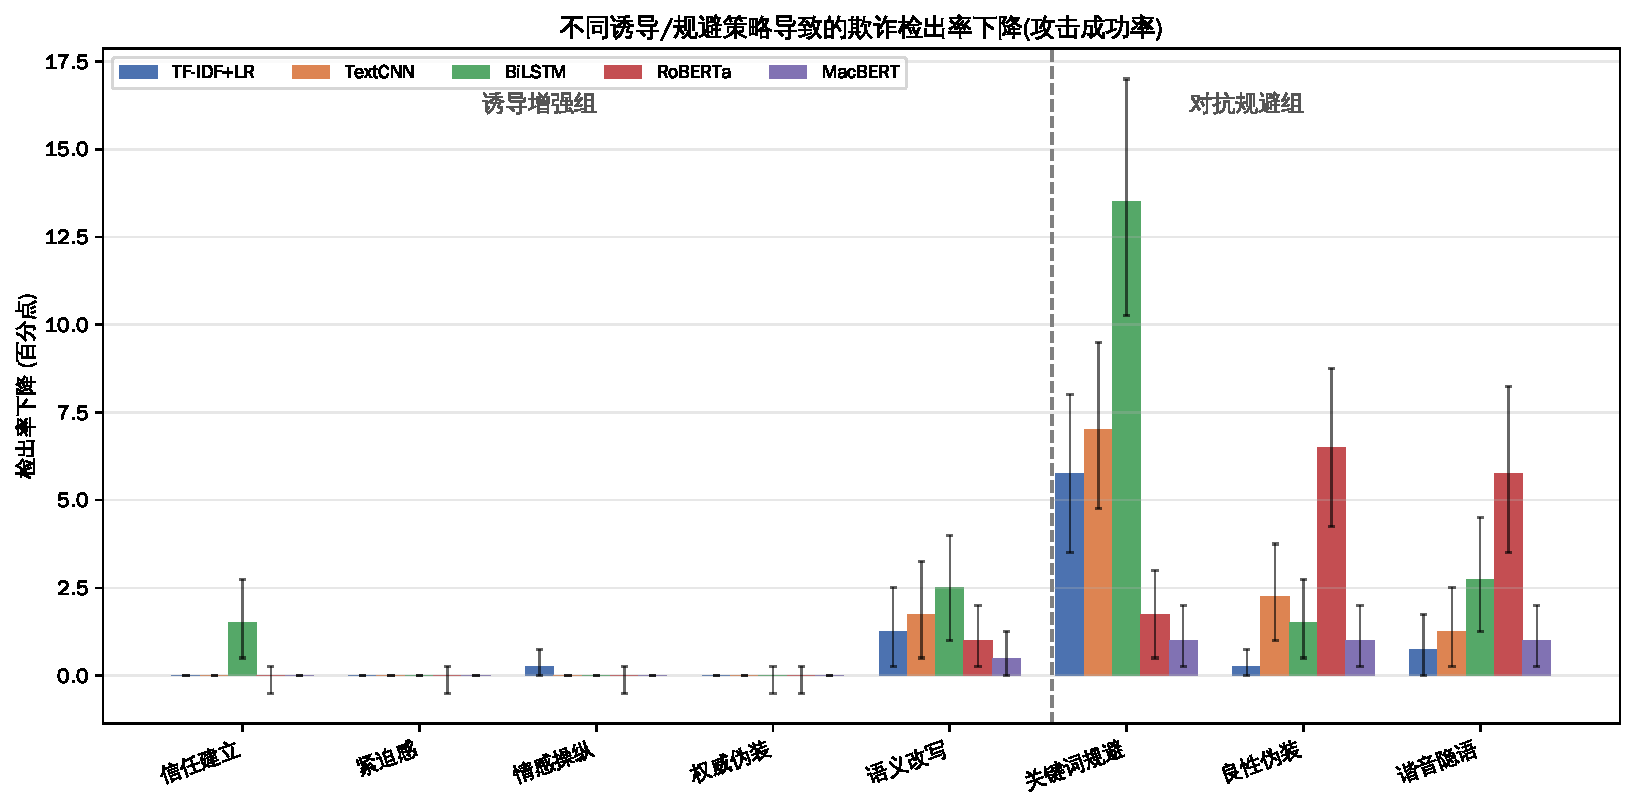
\includegraphics[width=0.92\textwidth]{figures/detection_drop.pdf}
\caption{不同策略导致的欺诈检出率下降(攻击成功率)。诱导增强组几乎不造成下降,对抗规避组(尤其关键词规避)造成显著下降。}
\label{fig:drop}
\end{figure}

\subsubsection{发现一:诱导增强策略几乎不削弱检测器,甚至适得其反}

从表~\ref{tab:robust} 左半部分可见,\textbf{信任建立、紧迫感、情感操纵、权威伪装}四种诱导增强策略对各模型检出率的影响微乎其微(普遍 $\leq$ 2.5 个百分点),多数情况下检出率维持在 99\%$\sim$100\%。对 RoBERTa,这些策略甚至使检出率\emph{略有上升}(从 99.8\% 升至 100.0\%)。

这一反直觉现象可由\textbf{关键词密度}的变化来解释。如表~\ref{tab:kw} 所示,信任建立、紧迫感、权威伪装等策略在增强对人的说服力的同时,显著\textbf{增加}了对话中欺诈关键词的数量(从原始的 3.21 个/通增至 6.7$\sim$7.3 个/通)。这些新增的"立即""冻结""官方""验证"等词,恰是检测器最敏感的判别特征——于是,使话术对人\emph{更具迷惑性}的修改,反而使其对检测器\emph{更易暴露}。这有力地验证了 §3.2.3 提出的\textbf{脆弱面正交性}假设:社会工程诱导针对的是人类的认知与情感弱点,而文本检测器作为冷静的旁观者并不受此影响。

\begin{table}[H]
\centering
\caption{不同改写策略下的平均欺诈关键词密度(个/通)与平均长度(字符)}
\label{tab:kw}
\scriptsize
\setlength{\tabcolsep}{3.5pt}
\begin{tabular}{l c | ccccc | ccc}
\toprule
& \textbf{原始} & 信任 & 紧迫 & 情感 & 权威 & 改写 & 规避 & 良性伪装 & 谐音隐语 \\
\midrule
关键词密度 & 3.21 & 6.74 & 7.26 & 2.61 & 6.78 & 2.19 & \textbf{0.73} & 4.89 & \textbf{0.67} \\
平均长度 & --- & 744 & 502 & 524 & 504 & 492 & 413 & 741 & 452 \\
\bottomrule
\end{tabular}
\end{table}

\subsubsection{发现二:对抗规避策略才能真正击穿检测器}

与诱导增强组形成鲜明对比,\textbf{对抗规避组}造成了显著的性能下降(表~\ref{tab:robust} 右半部分、图~\ref{fig:drop})。其中\textbf{关键词规避}策略威胁最大:它在保留欺诈意图的前提下,将关键词密度从 3.21 骤降至 0.73(表~\ref{tab:kw}),致使 BiLSTM 检出率从 99.8\% 跌至 86.2\%(下降 \textbf{13.5} 个百分点),TextCNN 下降 7.0 点,TF-IDF+LR 下降 5.8 点。\textbf{谐音隐语}策略同样有效(关键词密度降至 0.67),对 RoBERTa 造成 5.8 点下降。\textbf{良性伪装}则对 RoBERTa 影响最大(下降 6.5 点)——它用大段正常业务寒暄稀释诈骗信号,扰乱了模型对整体语义的判断。

这表明,\textbf{真正威胁检测器的不是"对人更狠"的诱导,而是"对机器更隐蔽"的规避}。这类攻击直接打击了检测器对表层特征的依赖,印证了 §1.4 指出的"对表层词汇线索的过度依赖"这一核心局限,也与 TextFooler~\cite{jin2020textfooler} 等对抗攻击研究的结论一致。

\subsubsection{发现三:模型鲁棒性呈现明显的代际分层}

综合所有策略,模型的鲁棒性排序为:\textbf{MacBERT $>$ RoBERTa $>$ TF-IDF+LR $\approx$ TextCNN $>$ BiLSTM}。预训练语言模型展现出最强的鲁棒性——MacBERT 在所有策略下检出率均不低于 99.0\%,即便面对最强的关键词规避也仅下降 1.0 点;这归功于其深层语义理解能力,能够透过表层用词捕捉"诱导转账/索取信息"的深层欺诈意图。相比之下,依赖局部 n-gram 与词频的浅层模型(BiLSTM、TextCNN、TF-IDF)在关键词被移除后性能明显滑坡。值得注意的是,RoBERTa 虽对关键词规避稳健,却对良性伪装与谐音隐语相对敏感,说明不同预训练模型存在差异化的脆弱面。

\subsubsection{发现四:置信度比硬标签更早暴露鲁棒性裂缝}

图~\ref{fig:conf} 给出了各模型平均欺诈置信度随策略的变化。即使在检出率(硬标签)尚未明显下降的情况下,\textbf{预测置信度已先行松动}。例如,对抗规避使 TF-IDF+LR 的平均置信度从 0.991 降至 0.856,BiLSTM 从 0.997 降至 0.858;语义改写、情感操纵亦使多数模型置信度下滑。这说明改写虽未必使样本越过 0.5 的决策阈值,却已将其推近边界——在更严苛的阈值或噪声叠加下,这些"勉强守住"的样本极可能失守。置信度因而是比准确率更敏感的鲁棒性探针。MacBERT 的置信度曲线最为平稳(始终 $\geq$ 0.99),再次印证其鲁棒性。

\begin{figure}[H]
\centering
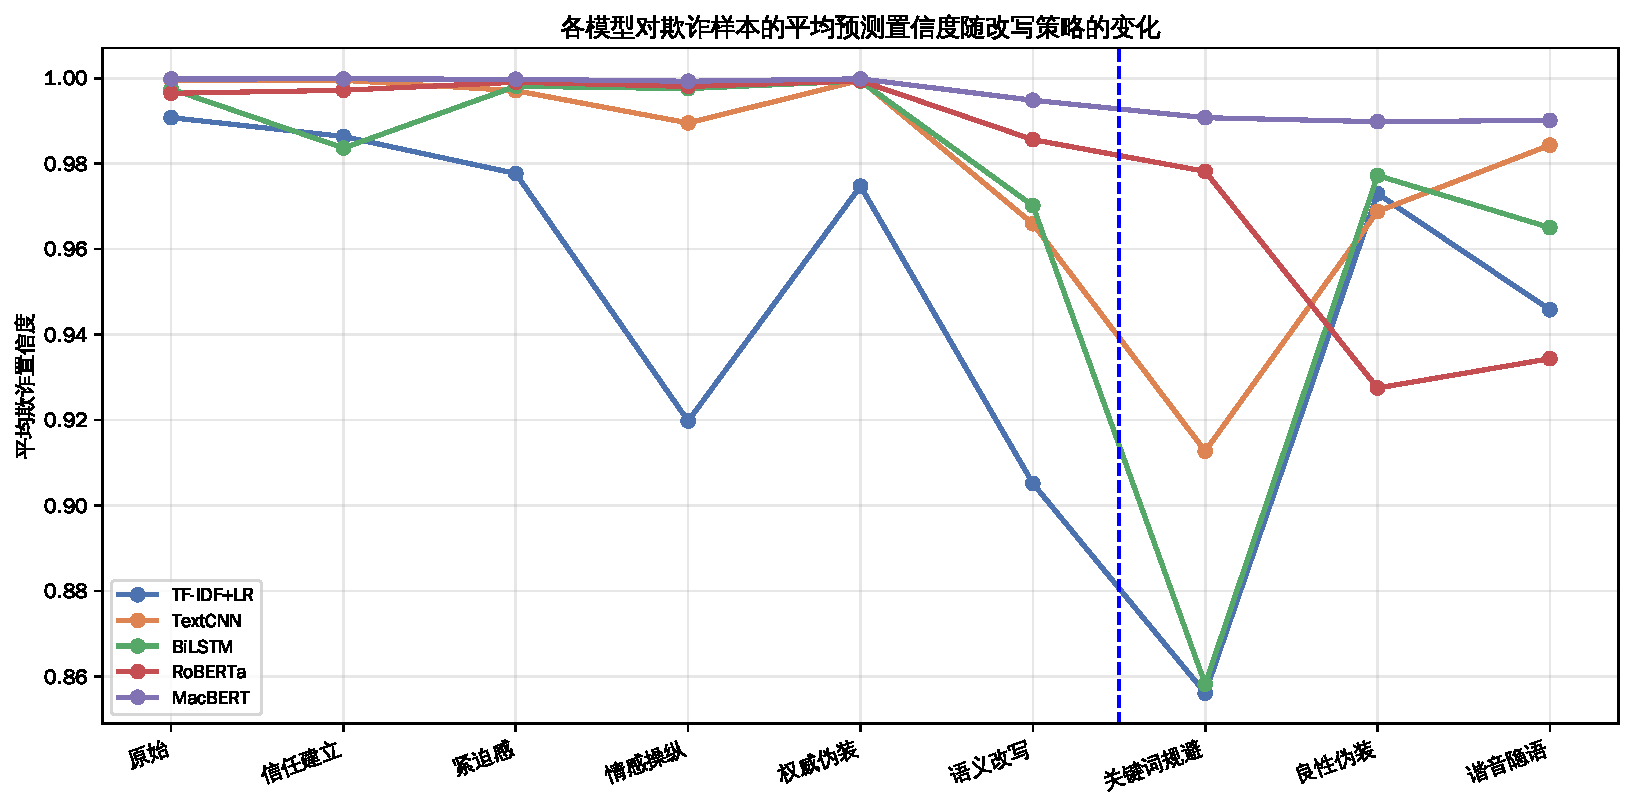
\includegraphics[width=0.9\textwidth]{figures/confidence_change.pdf}
\caption{各模型对欺诈样本的平均预测置信度随改写策略的变化。预训练模型曲线平稳,浅层模型在对抗规避组下置信度明显下滑。}
\label{fig:conf}
\end{figure}

\subsection{案例分析}

为直观说明对抗规避的作用机制,表~\ref{tab:case} 对比了同一条欺诈对话在关键词规避前后的片段。原文直白地出现"点击链接""验证码"等强信号,改写后则代之以"我发个东西给你,你点开按提示填""把那串数字念给我"等口语化、间接的表达——欺诈意图对人类而言依然清晰,但供检测器捕捉的关键词几乎被清除,从而成功规避了浅层模型的判别。

\begin{table}[H]
\centering
\caption{关键词规避改写前后的对话片段对比(节选)}
\label{tab:case}
\small
\begin{tabular}{p{2.0cm} p{12.5cm}}
\toprule
\textbf{版本} & \textbf{对话片段} \\
\midrule
原始 & ……为了保证您的权益,请您\textbf{点击我们发送的链接},按照提示操作即可完成退款……需要您提供\textbf{银行卡号}和\textbf{验证码}。 \\
\midrule
关键词规避 & ……给我一些您的基本情况,比如您\textbf{那个卡上的号}和我发过去的\textbf{一串数字}……我先加您微信,然后发个\textbf{小东西}给您,您\textbf{点开它,按上面的提示填一下}就行。 \\
\bottomrule
\end{tabular}
\end{table}

\subsection{讨论与启示}

本文实验得出三点对反诈系统设计具有指导意义的启示:

\begin{enumerate}[leftmargin=2em,itemsep=0.2em]
\item \textbf{高准确率可能是"虚假的安全感"}。在词汇可分性强的数据集上,简单模型即可达到近乎完美的精度,但这并不代表真实鲁棒性。评估反诈模型时,必须引入对抗改写测试,否则会系统性高估其防护能力。
\item \textbf{应优先采用具备深层语义理解的预训练模型}。MacBERT/RoBERTa 在对抗规避下的稳健性显著优于浅层模型,说明语义级建模是抵御关键词规避的有效途径。进一步地,可引入对抗训练~\cite{advtraining2024}、数据增强等手段强化鲁棒性。
\item \textbf{防御重心应对准"规避"而非"诱导"}。本文发现表明,检测器的脆弱性主要来自攻击者的特征隐藏行为(谐音、隐语、良性伪装),而非社会工程诱导本身。实战中应针对性地引入谐音归一化、隐语词典、语义意图识别等防御机制。
\end{enumerate}

\section{结论与展望}

本文围绕欺诈通话检测与鲁棒性评估,完成了两项核心工作。其一,构建了横跨传统机器学习、深度学习与预训练语言模型三个代际、共五种结构的中文欺诈通话分类模型,实验表明各模型在原始测试集上均可达到约 0.999$\sim$1.000 的 F1,但这种高性能高度依赖表层欺诈关键词。其二,借鉴 Fraud-R1 的多策略增强思想,设计了诱导增强与对抗规避两组共八种语义改写策略,并在不重训的前提下系统评估了各模型的鲁棒性。

核心结论为:\textbf{(1)} 以提升对人说服力为目标的社会工程诱导策略(信任、紧迫、情感、权威)几乎不削弱检测器,甚至因关键词密度上升而更易被检出,揭示了社会工程脆弱面与文本检测脆弱面的\textbf{正交性};\textbf{(2)} 真正击穿检测器的是以隐藏特征为目标的对抗规避策略,关键词规避使最脆弱的 BiLSTM 检出率下降达 13.5 个百分点;\textbf{(3)} 模型鲁棒性呈代际分层,具备深层语义理解的预训练模型(MacBERT、RoBERTa)远比浅层模型稳健;\textbf{(4)} 置信度是比硬标签更敏感的鲁棒性探针。

本研究亦存在局限:改写依赖单一大模型且样本规模有限,未来可扩大改写规模、引入多模型交叉改写,并探索对抗训练、谐音归一化等防御方法,以及多轮对话级的动态攻防评测,进一步逼近真实反诈对抗场景。

\section*{代码与数据}

本文的全部代码(数据预处理、五类模型训练、Fraud-R1 风格语义改写、鲁棒性评估与可视化)、实验结果与运行截图均已开源,详见 GitHub 仓库:

\begin{center}
\url{https://github.com/<your-username>/fraud-call-detection}
\end{center}

\bibliographystyle{unsrtnat}
\bibliography{references}

\end{document}



